\chapter{Bài 11. Một số lực trong thực tiễn}
\begin{center}
	\textit{(6 tiết)}
\end{center}
\section{MỤC TIÊU DẠY HỌC}
\begin{center}
	\begin{longtable}{|M{2.5cm}|L{12.5cm}|M{2cm}|}
		\hline
		\thead{Biểu hiện\\ năng lực} & \thead{Mục tiêu} & \thead{STT}\\
		\hline
		\multicolumn{3}{|c|}{\textbf{ Năng lực vật lí}}\\
		\hline
		1.1 & Nếu được khái niệm, công thức tính trọng lực. &1 \\
		\hline
		1.4 & Phân biệt được trọng lực và trọng lượng. &2 \\
		\hline
		1.1 & Nếu được khái niệm lực căng dây. &3 \\
		\hline
		1.1 & Nêu được những đặc điểm của lực ma sát nghỉ, ma sát trượt. &4 \\
		\hline
		1.1 & Viết được công thức tính độ lớn của lực ma sát trượt. &5 \\
		\hline
		1.5 & Mô tả được bằng các ví dụ thực tiễn và biểu diễn được lực ma sát. &6 \\
		\hline
			1.5 & Lấy được ví dụ về ích lợi và tác hại của lực ma sát trong đời sống. &7 \\
		\hline
		1.5 & Vận dụng kiến thức lực ma sát để giải thích một số hiện tượng trong thực tế. &8 \\
		\hline
		1.2 & Vận dụng đặc điểm của lực ma sát để giải các bài toán cơ bản. &9 \\
		\hline
		1.2 & Biểu diễn được lực cản, lực nâng trong trường hợp cụ thể.&10 \\
		\hline
		1.2 & Vận dụng đặc điểm của lực cản và lực nâng để giải một số bài toán đơn giản.&11 \\
		\hline
		\multicolumn{3}{|c|}{\textbf{Năng lực chung}}\\
		\hline
		TC - TH& Tích cực thực hiện các nhiệm vụ đặt ra cho nhóm khi tìm hiểu các lực trong thực tiễn.	& 12\\
		\hline
	\end{longtable}
\end{center}
\section{THIẾT BỊ DẠY HỌC VÀ HỌC LIỆU}
\begin{itemize}
	\item Tivi/máy chiếu;
	\item SGK.
\end{itemize}
\section{TIẾN TRÌNH DẠY HỌC}
\subsection{TIẾN TRÌNH}\begin{center}
	\begin{longtable}{|L{2.75cm}|C{1.25cm}|L{5cm}|L{3.5cm}|L{4cm}|}
		\hline
		\thead{Tiến trình} & \thead{Mục\\tiêu} & \thead{Nội dung dạy học \\trọng tâm} & \thead{PP,\\ KTDH} & \thead{Phương pháp \\đánh giá}\\
		\hline
		\textbf{Hoạt động 1:} Tìm hiểu về lực hấp dẫn và trọng lực& 1, 2, 12  & Định luật vạn vật hấp dẫn, khái niệm trọng lực, khái niệm trọng lượng  &PPDH: Thuyết trình  & GV đánh giá dựa trên câu trả lời của HS.\newline
		PP đánh giá: quan sát, nghe.  \\
		\hline
		\textbf{Hoạt động 2:} Tìm hiểu về lực ma sát trượt & 4, 5, 6, 7 & Lực ma sát trượt, biểu thức xác định độ lớn lực ma sát trượt &PPDH: Thuyết trình  & GV đánh giá dựa trên câu trả lời của HS.\newline
		PP đánh giá: quan sát, nghe.  \\
		\hline
		\textbf{Hoạt động 3:} Tìm hiểu về lực ma sát nghỉ và ma sát lăn& 4, 6, 7 & Lực ma sát nghỉ, lực ma sát lăn &PPDH: Thuyết trình  & GV đánh giá dựa trên câu trả lời của HS.\newline
		PP đánh giá: quan sát, nghe.  \\
		\hline
		\textbf{Hoạt động 4:} Vận dụng biểu thức xác định độ lớn lực ma sát trượt để giải các bài toán cơ bản& 5, 9, 12 & Vận dụng biểu thức xác định độ lớn lực ma sát trượt &PPDH: Đàm thoại  & GV đánh giá dựa trên bài tập ví dụ của HS.\newline
		PP đánh giá: quan sát, nghe.  \\
		\hline
		\textbf{Hoạt động 5:} Tìm hiểu về lực căng dây& 3, 12 & Đặc điểm lực căng dây, biểu diễn lực căng dây &PPDH: Thuyết trình  & GV đánh giá dựa trên câu trả lời của HS.\newline
		PP đánh giá: quan sát, nghe.  \\
		\hline
		\textbf{Hoạt động 6:} Tìm hiểu về lực đẩy Archimedes& 10, 11, 12 & Đặc điểm lực đẩy Archimedes &PPDH: Thuyết trình  & GV đánh giá dựa trên câu trả lời của HS.\newline
		PP đánh giá: quan sát, nghe.  \\
		\hline
		\textbf{Hoạt động 7:} Luyện tập	& 5, 9, 11 & Luyện tập bài tập động lực học. & PPDH:  Đàm thoại& GV đánh giá dựa trên bài tập cá nhân của học sinh.\newline
		PP đánh giá: quan sát, nghe. \\
		\hline
	\end{longtable}
\end{center}
\subsection{CÁC HOẠT ĐỘNG HỌC}
% ==========================================================================================
\hoatdong
{Tìm hiểu về lực hấp dẫn và trọng lực
}
{\begin{itemize}
		\item HS trình bày được biểu thức định luật vạn vật hấp dẫn.
		\item HS nêu được trọng lực là trường hợp riêng của lực hấp dẫn.
		\item HS phân biệt được trọng lực và trọng lượng.
	\end{itemize}
}
{Câu trả lời của HS cho các câu hỏi gợi mở của GV.
}
{\textit{\underline{* GV chuyển giao nhiệm vụ học tập}}
	\begin{itemize}[label=-]
		\item GV giới thiệu chuyển động của các hành tinh xung quanh Mặt Trời, vệ tinh xung quanh Trái Đất, vật trên Trái Đất khi thả thì rơi xuống đất đều nhờ vào tác dụng của lực hấp dẫn. Mọi vật trong vũ trụ đều đang tương tác với nhau bằng lực hấp dẫn.
		\begin{center}
			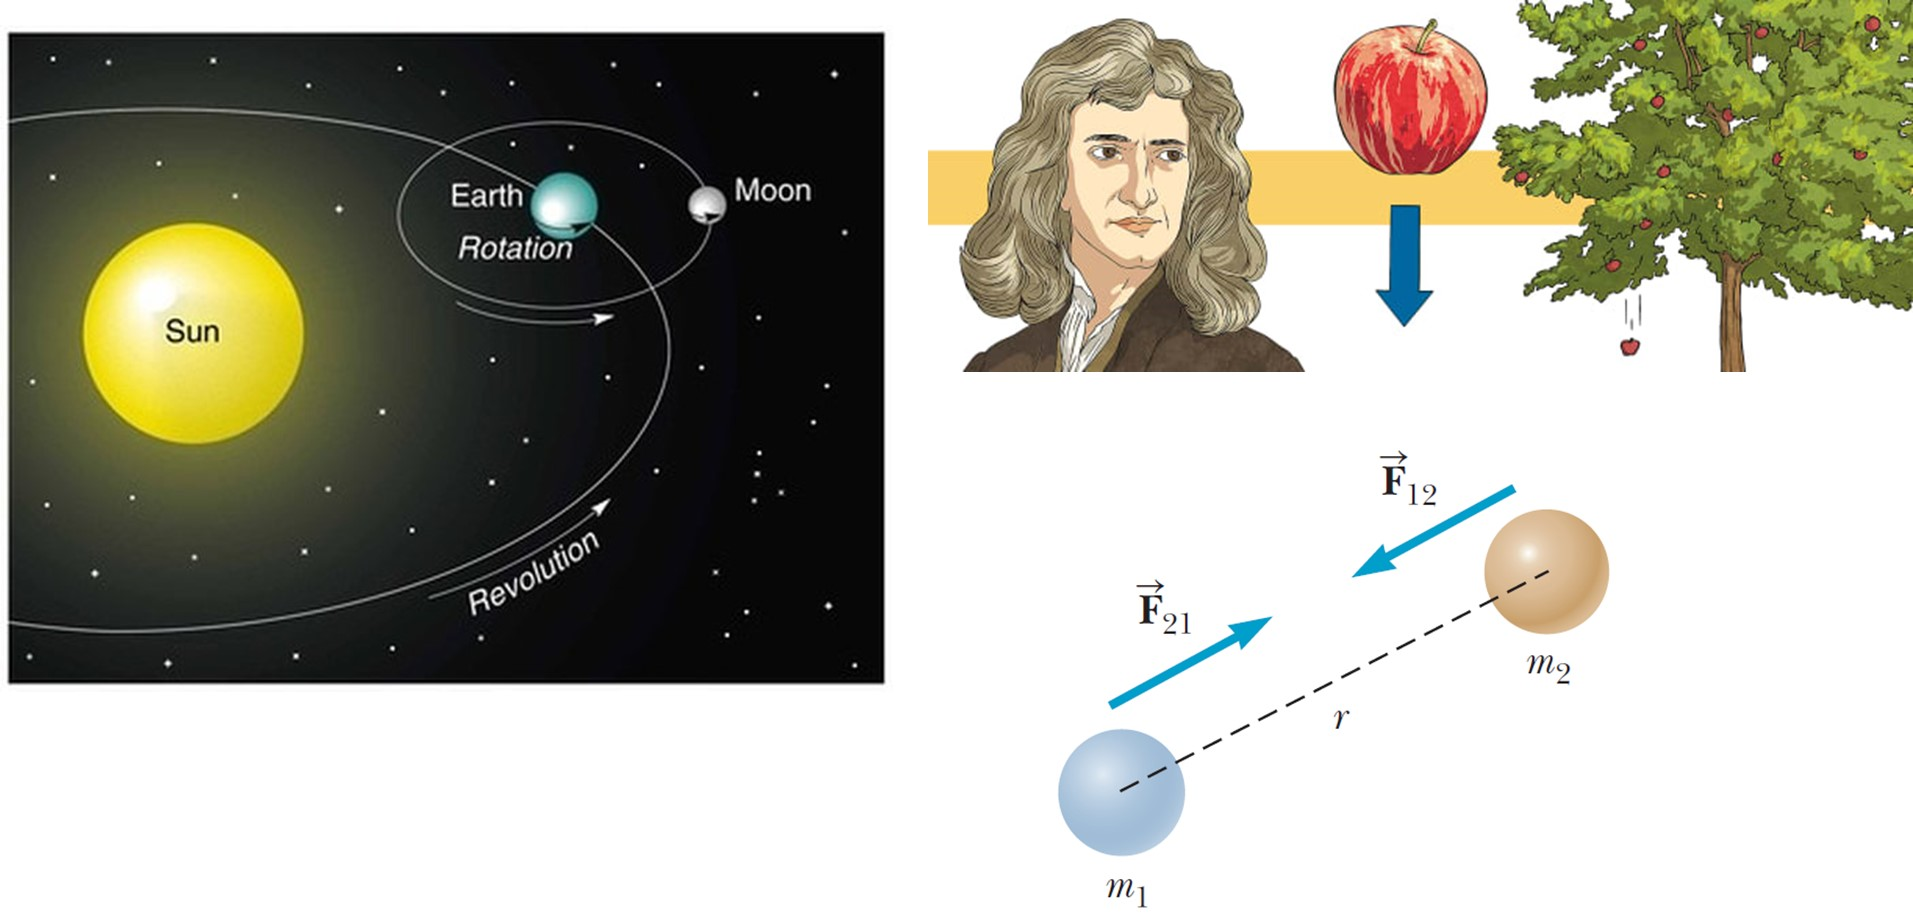
\includegraphics[scale=0.4]{figs/G10-BAI11-1}
		\end{center}
		\item GV giới thiệu cho HS về định luật vạn vật hấp dẫn.
		\item GV giới thiệu cho HS về giới hạn sử dụng định luật vạn vật hấp dẫn:
		\begin{itemize}[label=$\bullet$]
			\item Định luật áp dụng với trường hợp khoảng cách giữa các vật rất lớn so với kích thước giữa chúng (chất điểm).
			\item Hai vật đồng chất, hình cầu thì $r$ là khoảng cách nối tâm 2 vật. Lực hấp dẫn trùng phương nối tâm và có điểm đặt tại tâm mỗi vật.
		\end{itemize}
		\item GV giới thiệu cho HS trọng lực là trường hợp riêng của lực hấp dẫn. Từ đó, GV hướng dẫn HS xây dựng biểu thức gia tốc trọng trường.
		\item GV đặt câu hỏi: \textit{"Dựa vào biểu thức gia tốc trọng trường em hãy cho biết gia tốc trọng trường phụ thuộc vào các yếu tố nào?"}
		\item GV giới thiệu cho HS khái niệm trọng lượng: Trọng lượng là số chỉ của dụng cụ đo (dụng cụ xác định trọng lực hoặc khối lượng). Trong một số tình huống, trọng lực và trọng lượng có giá trị khác nhau.
		\item GV yêu cầu HS thực hiện ví dụ 1.
	\end{itemize}
		\textit{\underline{* HS thực hiện nhiệm vụ học tập}}
	\begin{itemize}[label=-]
		\item HS chú ý lắng nghe, đặt câu hỏi.
		\item HS hoạt động cá nhận để thực hiện ví dụ 1.
	\end{itemize}
	\textit{\underline{* HS báo cáo kết quả nhiệm vụ học tập}}
	\begin{itemize}[label=-]
		\item GV mời 1 HS lên bảng trình bày kết quả ví dụ 1.
		\item Các HS khác theo dõi và nhận xét.
		\item GV chỉnh lí và hợp thức hóa kiến thức.
	\end{itemize}
}
% ==========================================================================================
\hoatdong
{Tìm hiểu về lực ma sát trượt.
}
{\begin{itemize}
		\item HS trình bày được đặc điểm của lực ma sát trượt.
		\item HS viết được biểu thức xác định độ lớn của lực ma sát trượt.
	\end{itemize}
}
{Kết quả báo cáo thí nghiệm của các nhóm HS.
}
{	\textit{\underline{* GV chuyển giao nhiệm vụ học tập}}
	\begin{itemize}[label=-]
		\item GV đặt câu hỏi gợi mở vấn đề: Trong các trường hợp phanh xe gấp, bánh xe sẽ để lại vết trượt đen dài trên đường. Điều này là do đâu?
		\begin{center}
			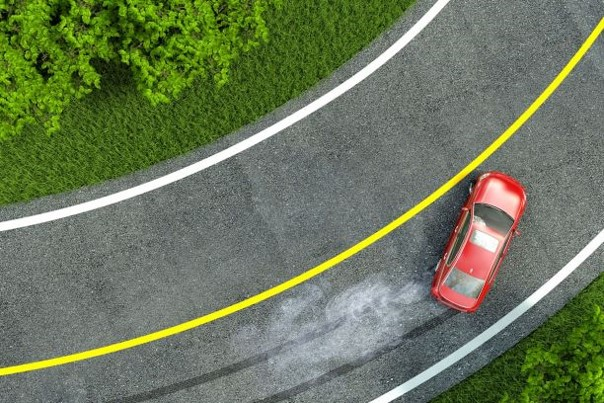
\includegraphics[scale=0.4]{figs/G10-BAI11-2}
		\end{center}
		\item GV giới thiệu cho HS bản chất của lực ma sát trượt là do lực tương tác tĩnh điện giữa 2 bề mặt tiếp xúc khi cọ xát với nhau.
		\begin{center}
			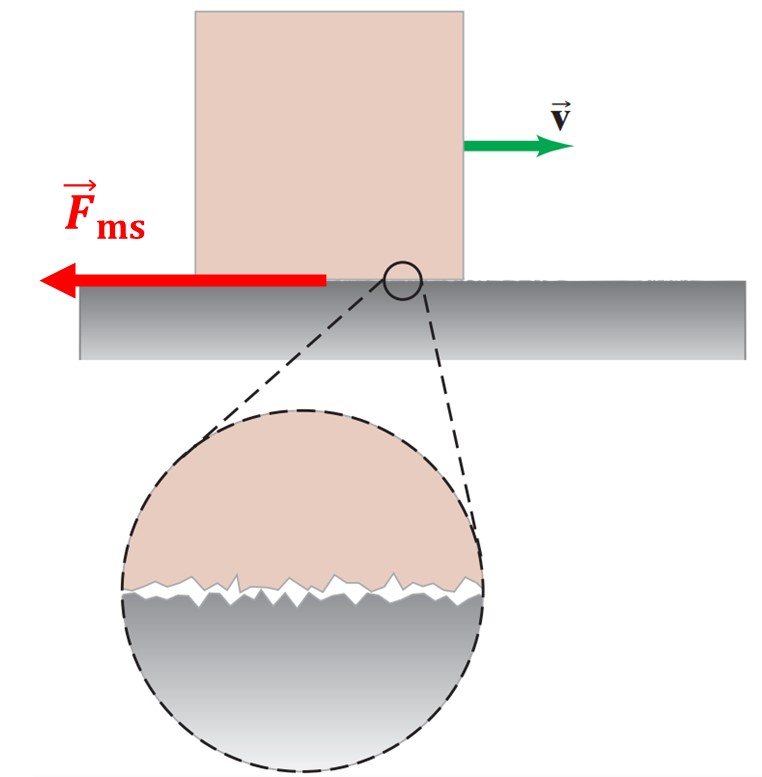
\includegraphics[scale=0.5]{figs/G10-BAI11-3}
		\end{center}
		\item Dựa vào kiến thức về tương tác tĩnh điện mà HS đã học ở chương trình KHTN, GV yêu cầu HS dự đoán về hướng của lực ma sát trượt.
		\item GV chia lớp thành 6 nhóm và giao cho các nhóm thực hiện 2 thí nghiệm sau (Nhóm 1, 2, 3 thực hiện thí nghiệm 1 và Nhóm 4, 5, 6 thực hiện thí nghiệm 2):
		\begin{itemize}[label=$\bullet$]
			\item \textbf{THÍ NGHIỆM 1:} \textit{Khảo sát sự phụ thuộc của lực ma sát vào vật liệu và tình trạng bề mặt tiếp xúc.}\\
			\textbf{\textit{Dụng cụ:}} Lực kế (có GHĐ \SI{1.0}{\newton} và ĐCNN \SI{0.01}{\newton}), khối gỗ hình hộp chữ nhật, các bề mặt: gỗ, giấy, inox.\\
			\textbf{\textit{Tiến hành:}}
			\begin{center}
				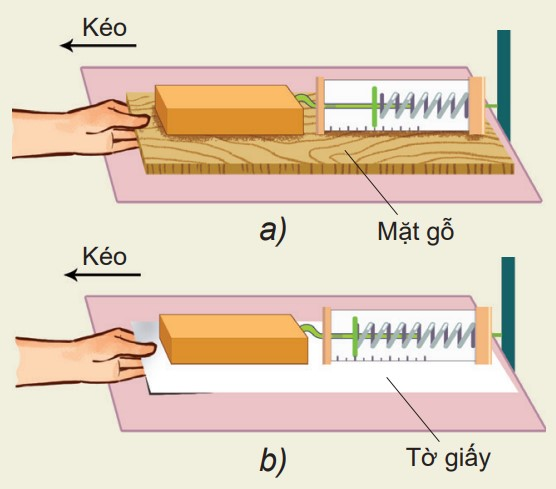
\includegraphics[scale=0.7]{figs/G10-BAI11-4.jpg}
			\end{center}
			\begin{itemize}
				\item Gắn lực kế vào giá thí nghiệm để cố định lực kế theo phương nằm ngang.
				\item Móc khối gỗ vào lực kế, lần lượt kéo các mặt tiếp xúc (mặt gỗ, mặt tờ giấy, mặt inox) theo phương nằm ngang để chúng trượt đều dưới khối gỗ.
				\item Ghi số chỉ của lực kế vào bảng bên dưới. Lấy giá trị trung bình của các số chỉ lực kế làm độ lớn của lực ma sát trượt.
				\begin{center}
					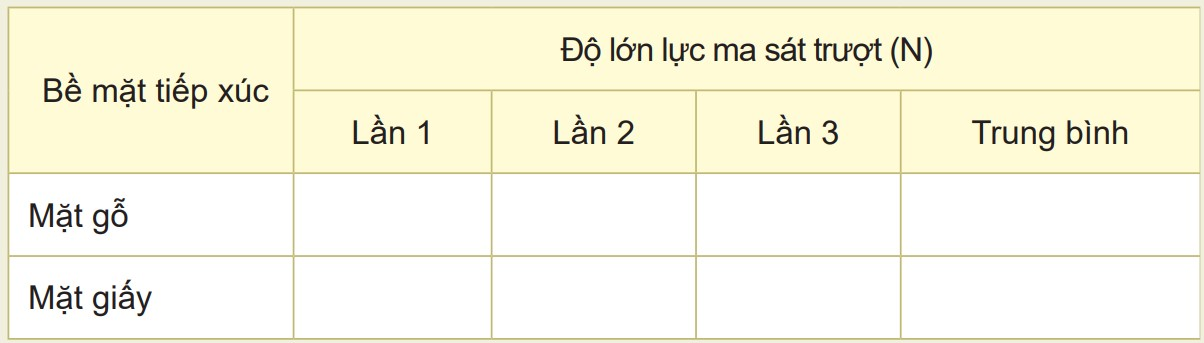
\includegraphics[scale=0.55]{figs/G10-BAI11-5}
				\end{center}
			\end{itemize}
				\textbf{\textit{Thảo luận và phân tích:}}
				\begin{itemize}
					\item Nêu các lực tác dụng lên khối gỗ khi mặt tiếp xúc bên dưới nó được kéo trượt đều. Tại sao khi đó số chỉ của lực kế bằng độ lớn của lực ma sát trượt?
					\item Sắp xếp thứ tự theo mức tăng dần lực ma sát trên mỗi bề mặt.
				\end{itemize}
			\item \textbf{THÍ NGHIỆM 2:} \textit{Khảo sát mối liên hệ giữa độ lớn của lực ma sát trượt với độ lớn của áp lực lên bề mặt tiếp xúc.}\\
			\textbf{\textit{Dụng cụ:}} Lực kế (có GHĐ \SI{1.0}{\newton} và ĐCNN \SI{0.01}{\newton}), ba khối gỗ hình hộp chữ nhật giống nhau, mặt tiếp xúc: gỗ.\\
			\textbf{\textit{Tiến hành:}}
			\begin{itemize}
				\item Đo trọng lượng của khối gỗ bằng lực kế.
				\item Gắn lực kế vào giá thí nghiệm để cố định lực kế theo phương nằm ngang.
				\item Móc khối gỗ vào lực kế, kéo mặt tiếp xúc (mặt gỗ) theo phương nằm ngang để nó trượt đều dưới khối gỗ. Ghi lại số chỉ của lực kế trong 3 lần thí nghiệm vào bảng bên dưới. Lấy giá trị trung bình các kết quả đo.
				\item Lần lượt đặt thêm 1, 2 khối gỗ lên trên khối gỗ đầu tiên và lặp lại bước 3.
				\begin{center}
					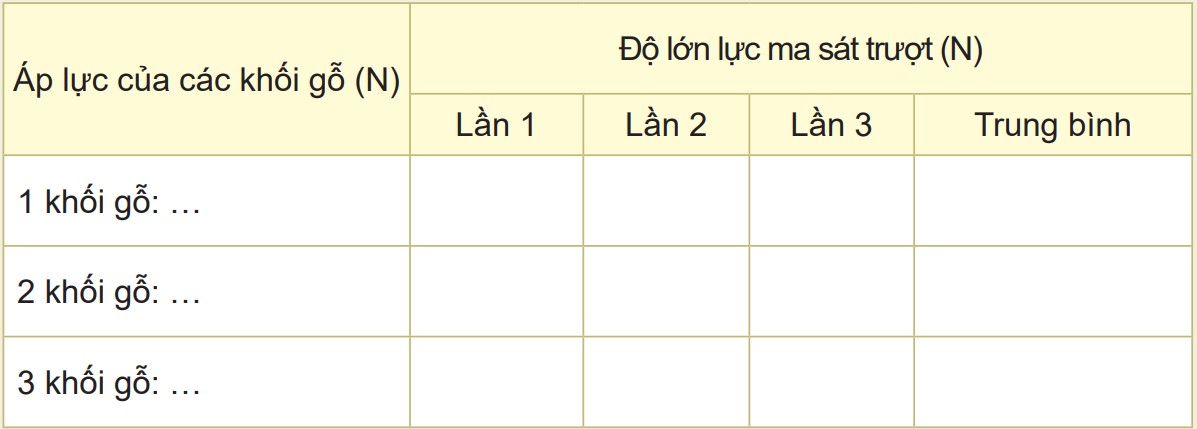
\includegraphics[scale=0.5]{figs/G10-BAI11-6}
				\end{center}
			\end{itemize}
			\textbf{\textit{Thảo luận và phân tích:}}
			\begin{itemize}
				\item Điều gì xảy ra với độ lớn của lực ma sát trượt khi tăng áp lực lên bề mặt tiếp xúc?
				\item Vẽ đồ thị cho thấy sự thay đổi độ lớn của lực ma sát trượt khi tăng dần độ lớn của áp lực.
			\end{itemize}
		\end{itemize}
		\item GV theo dõi, hỗ trợ HS trong quá trình các nhóm thực hiện thí nghiệm.
		
	\end{itemize}
	\textit{\underline{* HS thực hiện nhiệm vụ học tập}}
	\begin{itemize}[label=-]
		\item HS chú ý lắng nghe.
		\item HS hoạt động theo nhóm để thực hiện thí nghiệm.
	\end{itemize}
	\textit{\underline{* HS báo cáo kết quả nhiệm vụ học tập}}
	\begin{itemize}[label=-]
		\item Các nhóm nộp lại báo cáo thí nghiệm cho GV.
		\item GV mời đại diện 2 nhóm HS (2 nhóm thực hiện 2 thí nghiệm độc lập) báo cáo kết quả thí nghiệm của nhóm.
		\item GV yêu cầu HS kết luận về những đặc điểm về độ lớn của lực ma sát trượt.
		\item GV nhận xét, chuẩn hóa kiến thức.
	\end{itemize}
}
% ==========================================================================================
\hoatdong
{Tìm hiểu về lực ma sát nghỉ và ma sát lăn.
}
{\begin{itemize}
		\item HS nêu được đặc điểm của lực ma sát nghỉ và ma sát lăn.
		\item HS trình bày được lợi ích và tác hại của lực ma sát trong đời sống.
	\end{itemize}
}
{Câu trả lời của HS về lực ma sát nghỉ, ma sát lăn, lợi ích và tác hại của lực ma sát.
}
{\textit{\underline{* GV chuyển giao nhiệm vụ học tập}}
	\begin{itemize}[label=-]
		\item GV đặt ra tình huống có vấn đề: GV dùng 1 tay ép cuốn sách lên bảng, GV yêu cầu HS xác định các lực tác dụng lên quyển sách.
		\begin{center}
			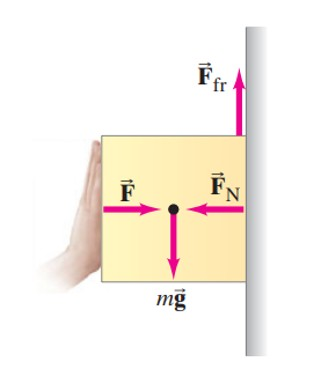
\includegraphics[scale=0.5]{figs/G10-BAI11-7}
		\end{center}
		\item GV đặt câu hỏi: \textit{"Nếu trên phương thẳng đứng quyển sách chỉ chịu tác dụng của trọng lực thì quyển sách có thể cân bằng được không?"}
		\item GV giới thiệu lực đang cân bằng với trọng lực trên phương thẳng đứng là lực ma sát nghỉ.
		\item GV đưa ra thêm tình huống người đang đẩy vật nặng trên sàn nhưng vật chưa chuyển động, GV yêu cầu HS xác định phương chiều của lực ma sát nghỉ lúc này.
		\begin{center}
			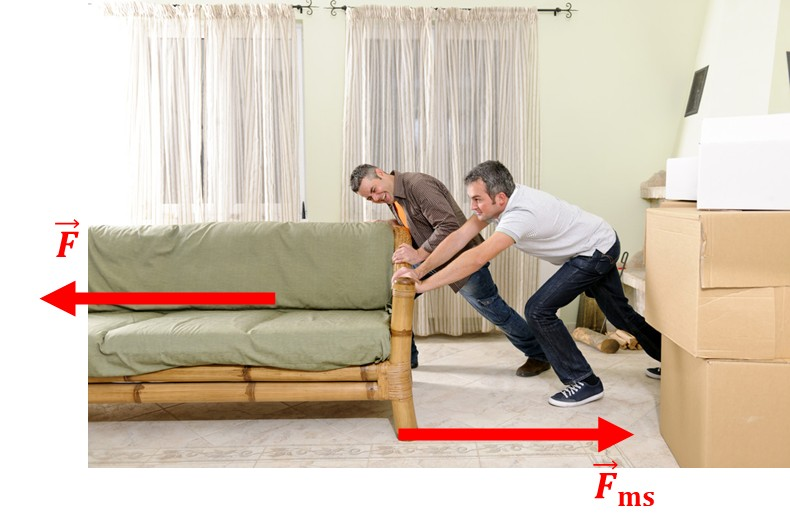
\includegraphics[scale=0.5]{figs/G10-BAI11-8}
		\end{center}
		\item Từ các tình huống trên, GV yêu cầu HS tổng quát lên điều kiện xuất hiện và đặc điểm của lực ma sát nghỉ.
		\item GV giới thiệu: Thông thường, lực ma sát nghỉ cực đại lớn hơn lực ma sát trượt.
		\begin{center}
			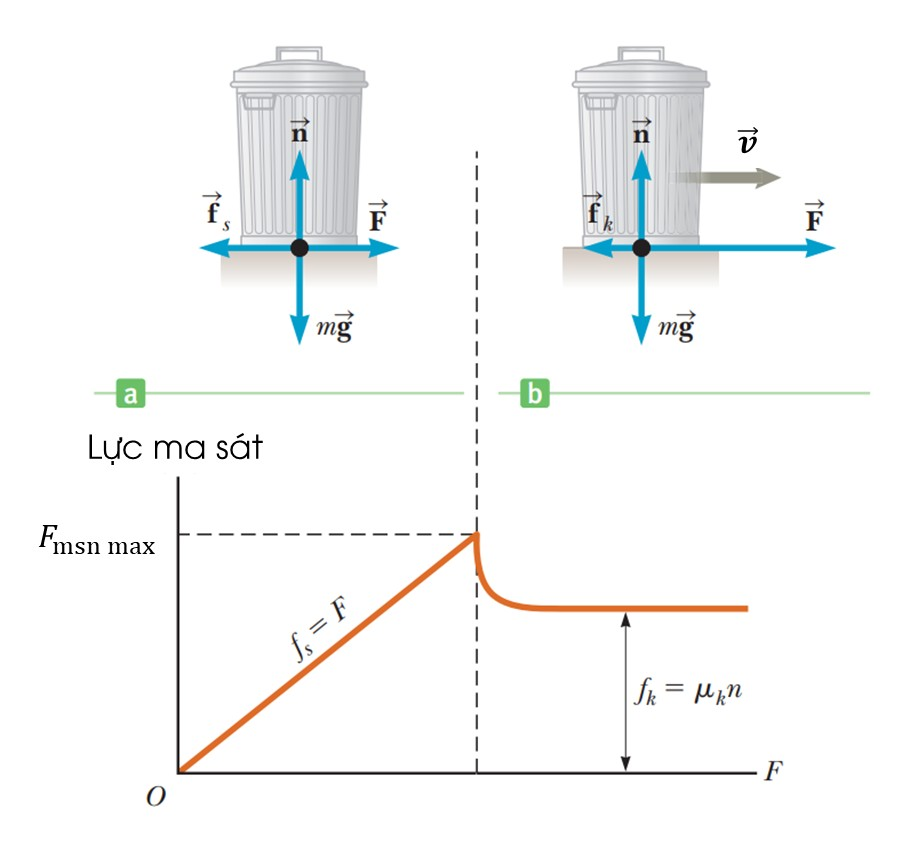
\includegraphics[scale=0.7]{figs/G10-BAI11-9}
		\end{center}
		\item GV đặt câu hỏi: \textit{"Vậy lực ma sát nói chung là có lợi hay có hại? Em hãy cho ví dụ để chứng minh khẳng định của mình."}
	\end{itemize}
	\textit{\underline{* HS thực hiện nhiệm vụ học tập}}\\
	HS chú ý lắng nghe và tích cực trả lời các câu hỏi gợi ý của GV.\\
	\textit{\underline{* HS báo cáo kết quả nhiệm vụ học tập}}
	\begin{itemize}[label=-]
		\item GV mời HS trả lời các câu hỏi gợi mở.
		\item Cả lớp lắng nghe, nhận xét.
		\item GV chỉnh lí, chuẩn hóa kiến thức.
	\end{itemize}
	
}
% ==========================================================================================
\hoatdong
{Vận dụng biểu thức xác định độ lớn lực ma sát trượt để giải các bài toán cơ bản.
}
{HS vận dụng được biểu thức xác định độ lớn lực ma sát trượt.
}
{Kết quả bài tập ví dụ của HS.
}
{\textit{\underline{* GV chuyển giao nhiệm vụ học tập}}
	\begin{itemize}[label=-]
		\item GV nhắc lại định luật II Newton, biểu thức xác định độ lớn lực ma sát trượt, đặc điểm của lực ma sát trượt.
		\item GV lần lượt chuyển giao các bài tập ví dụ 1 - 3 cho HS.
	\end{itemize}
	\textit{\underline{* HS thực hiện nhiệm vụ học tập}}\\
	HS chú ý lắng nghe và tích cực trả lời các câu hỏi gợi ý của GV.\\
	HS thực hiện Ví dụ 1 đến Ví dụ 3.\\
	\textit{\underline{* HS báo cáo kết quả nhiệm vụ học tập}}\\
	GV lần lượt mời HS trả lời câu hỏi và lên bảng giải bài tập Ví dụ.
}
% ==========================================================================================
\hoatdong
{Tìm hiểu về lực căng dây.
}
{HS nêu được đặc điểm của lực căng dây.
}
{Câu trả lời của HS về đặc điểm của lực căng.
}
{\textit{\underline{* GV chuyển giao nhiệm vụ học tập}}
	\begin{itemize}[label=-]
		\item GV yêu cầu HS xác định lực do dây chun tác dụng lên 2 đầu ngón tay có phương và chiều thế nào?
		\begin{center}
			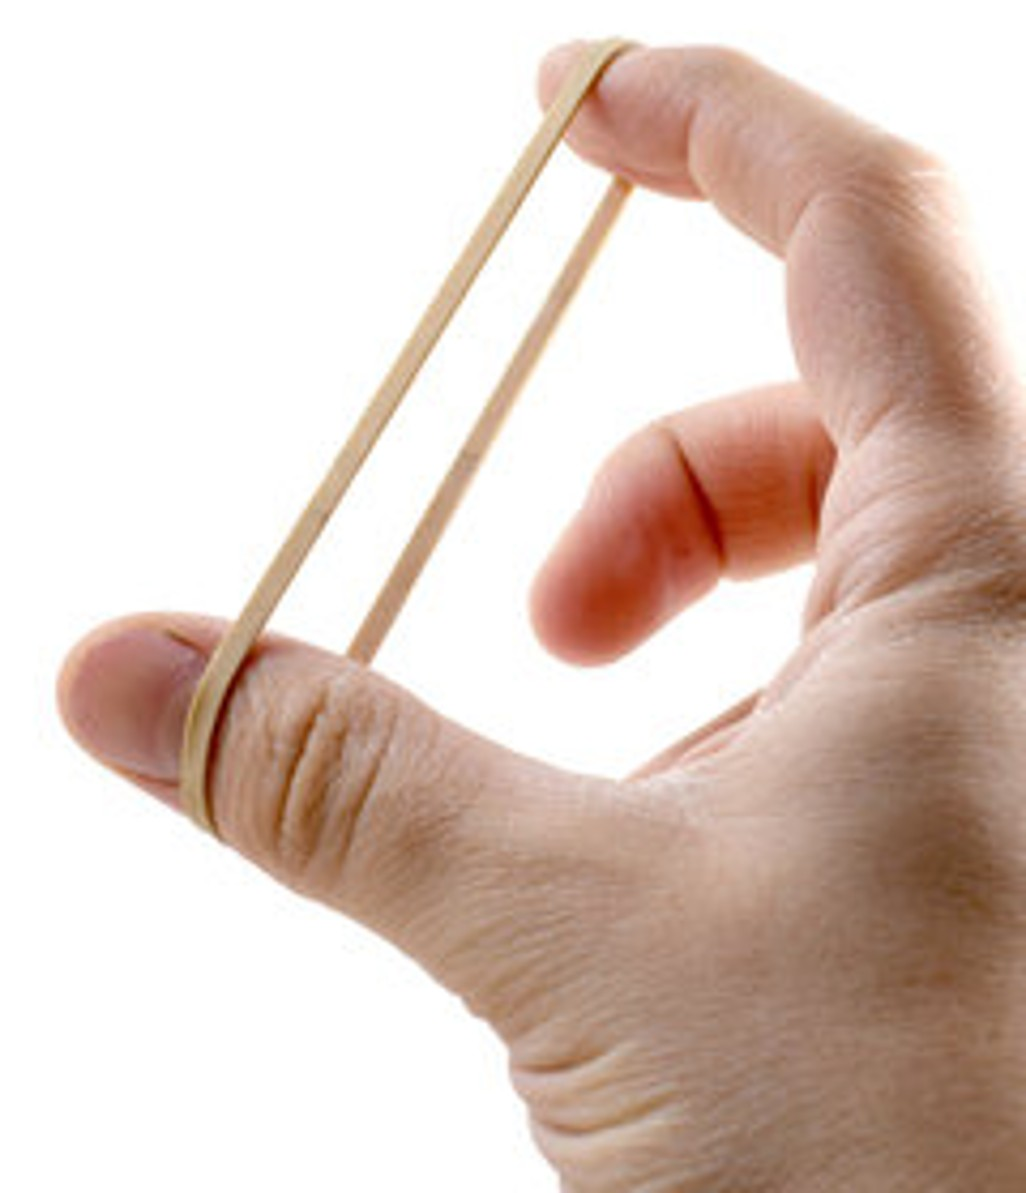
\includegraphics[scale=0.4]{figs/G10-BAI11-10}
		\end{center}
		\item Từ câu trả lời của HS, GV tổng quát lại các đặc điểm của lực căng dây.\\
		Khi một sợi dây bị kéo căng, sẽ có lực tác dụng lên hai vật gắn với hai đầu dây, lực căng dây có đặc điểm:
		\begin{itemize}[label=$\bullet$]
			\item điểm đặt là điểm mà đầu dây tiếp xúc với vật;
			\item phương của lực là phương của sợi dây;
			\item chiều hướng từ hai đầu dây vào điểm giữa của sợi dây.
		\end{itemize}
		Với những dây có khối lượng không đáng kể thì lực căng ở hai đầu dây luôn có cùng độ lớn.
		\item GV yêu cầu HS xác định lực căng dây trong trường hợp vật nặng được treo trên sợi dây mảnh, không dãn.
		\begin{center}
			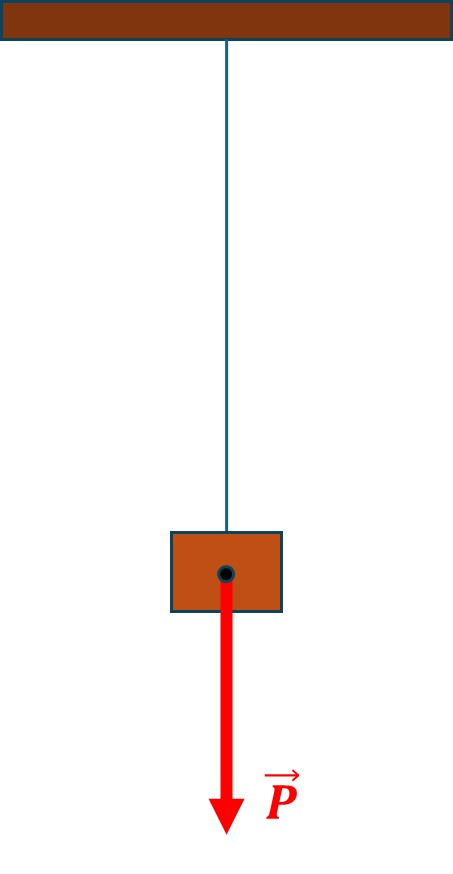
\includegraphics[scale=0.4]{figs/G10-BAI11-11}
		\end{center}
		\item 	GV hướng dẫn HS cách giải bài toán cân bằng của vật treo bằng dây nhẹ, không dãn.\\
			Vật ở trạng thái cân bằng lực khi tổng hợp lực tác dụng lên vật bằng không:
			$$\sum\vec{F}=\vec{0}\hspace{0.5cm} (*)$$
			Để giải phương trình (*), thông thường có thể sử dụng 2 cách:
			\begin{itemize}
				\item \textbf{Cách 1:} Chọn hệ trục tọa độ vuông góc $Oxy$ rồi chiếu phương trình (*) lên các trục $Ox$ và $Oy$ tương ứng.
				\item \textbf{Cách 2:} Sử dụng quy tắc đa giác vector.
			\end{itemize}
			\item GV chuyển giao HS thực hiện Ví dụ 4.
	\end{itemize}
	\textit{\underline{* HS thực hiện nhiệm vụ học tập}}\\
	HS chú ý lắng nghe và tích cực trả lời các câu hỏi gợi ý của GV.\\
	HS thực hiện Ví dụ 4.\\
	\textit{\underline{* HS báo cáo kết quả nhiệm vụ học tập}}\\
	GV lần lượt mời HS trả lời câu hỏi và lên bảng giải bài tập Ví dụ 4.
}
% ==========================================================================================
\hoatdong
{Tìm hiểu về lực đẩy Archimedes.
}
{\begin{itemize}
		\item HS biểu diễn được lực nâng của chất lưu.
		\item HS vận dụng được đặc điểm lực nâng của chất lưu để giải một số bài toán đơn giản.
	\end{itemize}
}
{Phần trả lời câu hỏi vận dụng của HS.
}
{\textit{\underline{* GV chuyển giao nhiệm vụ học tập}}
	\begin{itemize}[label=-]
		\item GV nhắc lại khái niệm khối lượng mà HS đã được học trong chương trình KHTN.\\
		Khối lượng riêng của một chất được xác định bằng khối lượng của một đơn vị thể tích chất đó 
		$$\rho=\dfrac{m}{V}.$$
		\begin{center}
			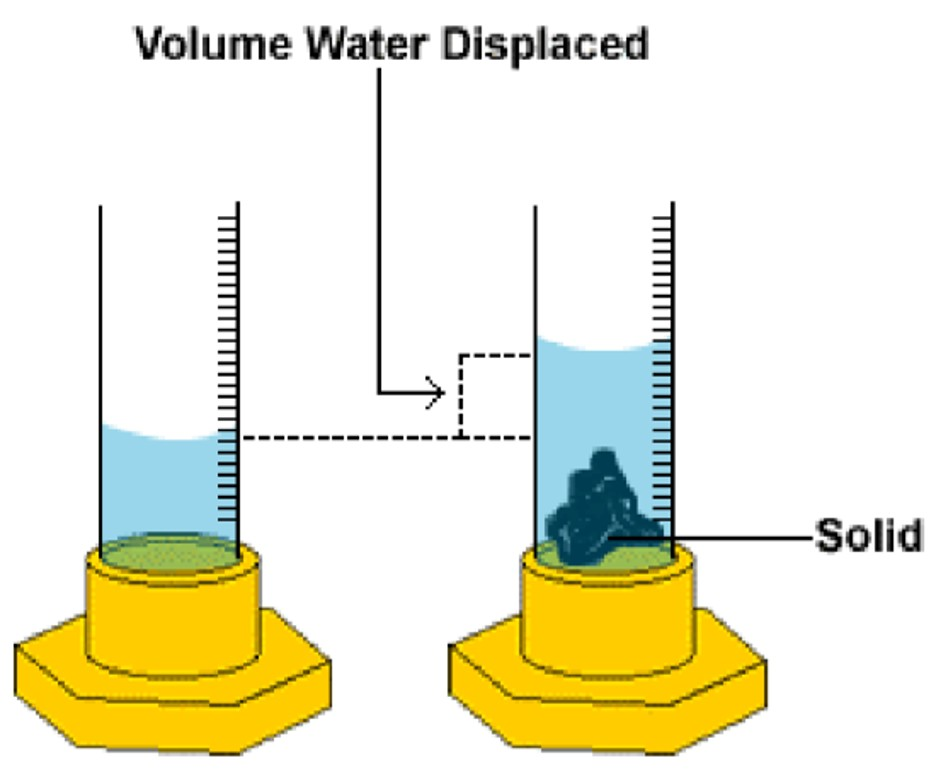
\includegraphics[scale=0.5]{figs/G10-BAI11-12}
		\end{center}
		\item GV đặt ra vấn đề nghiên cứu: Từ xa xưa, khi khai thác gỗ ở thượng nguồn thì người xưa đã biết cách kết gỗ thành bè và thả trôi về hạ nguồn. Người xưa đã vận dụng vào đặc điểm nào của nước?
		\begin{center}
			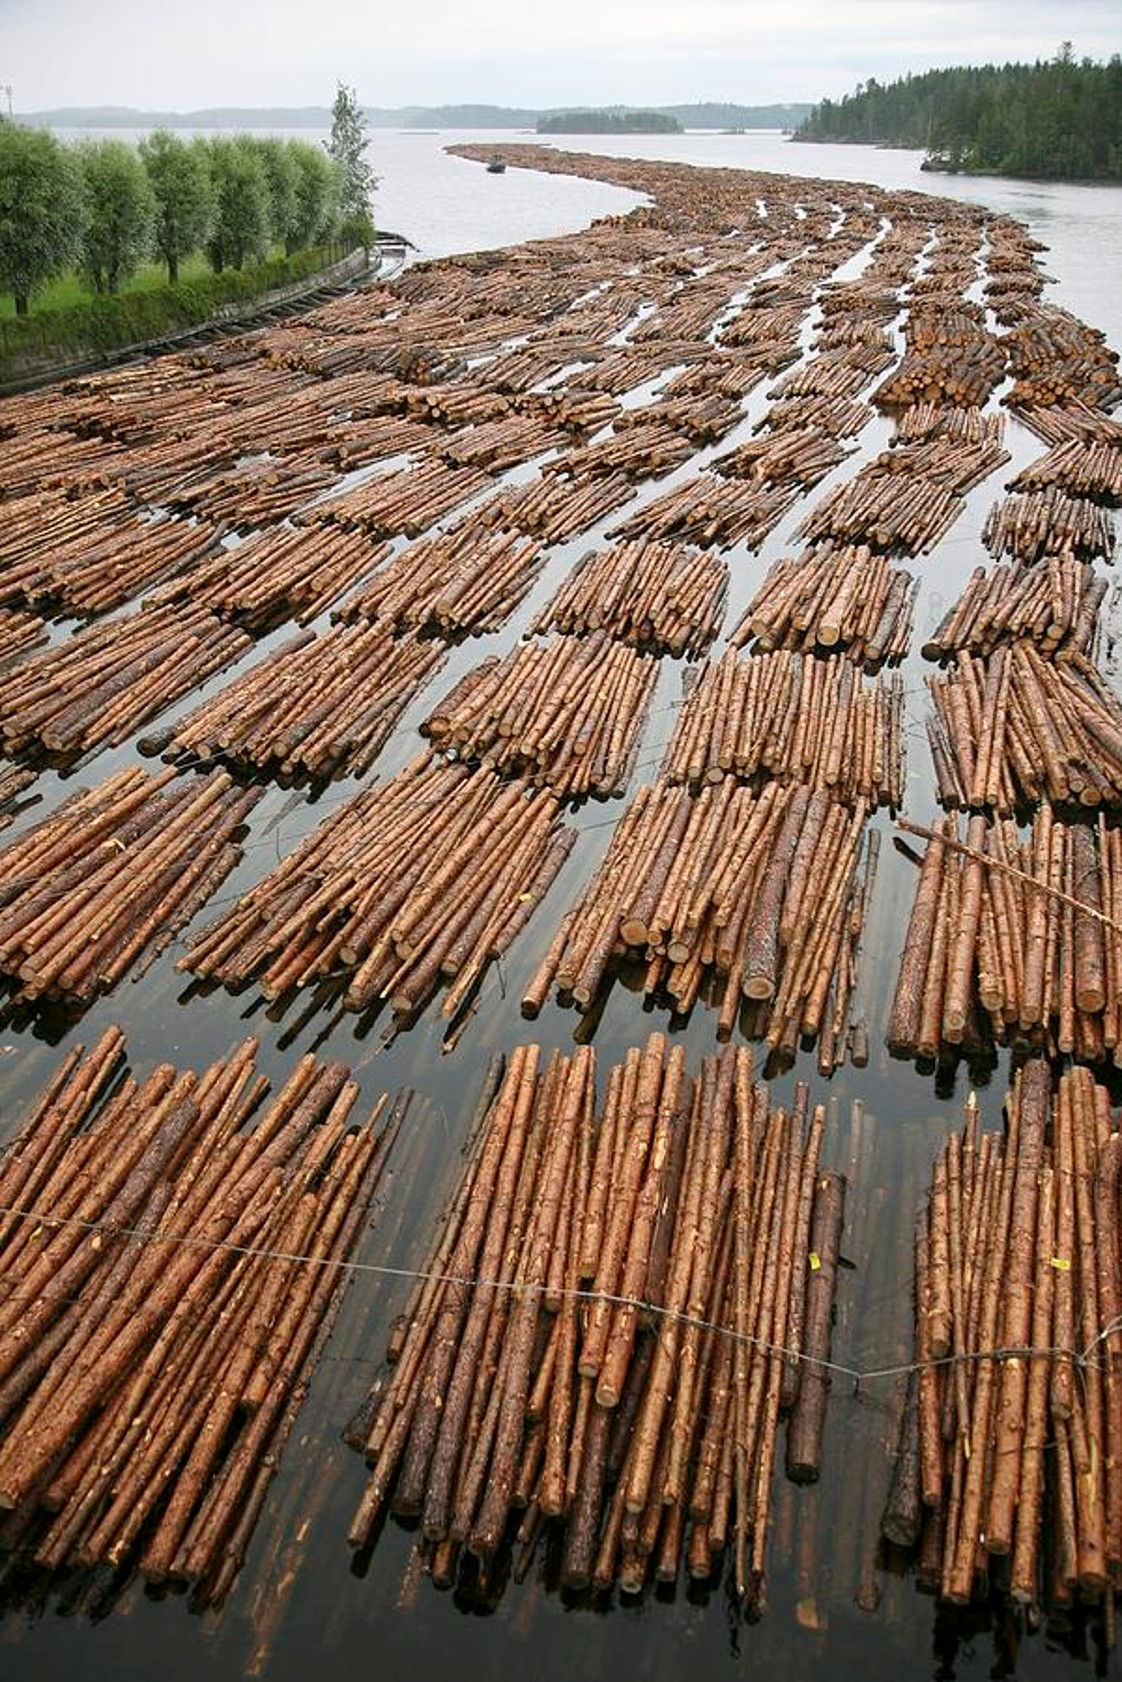
\includegraphics[scale=0.5]{figs/G10-BAI11-13}
		\end{center}
		\item GV hướng dẫn HS xác định biểu thức lực đẩy Archimedes.\\
		Xét một khối chất lỏng hình lập phương đang ở trong một bình chất lỏng (cùng loại) và đứng yên. Khối chất lỏng này chịu tác dụng của các lực nào?
		\begin{center}
			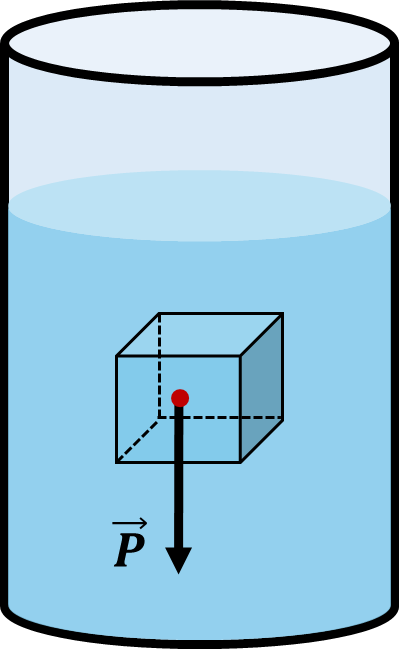
\includegraphics[scale=0.5]{figs/G10-BAI11-14}
		\end{center}
		GV đặt câu hỏi: \textit{"Trọng lượng khối chất lỏng này được xác định thế nào?"}\\
		GV đặt câu hỏi: \textit{"Để khối chất lỏng đứng yên thì chất lỏng xung quanh phải tác dụng lực lên nó thế nào?"}
		\begin{center}
			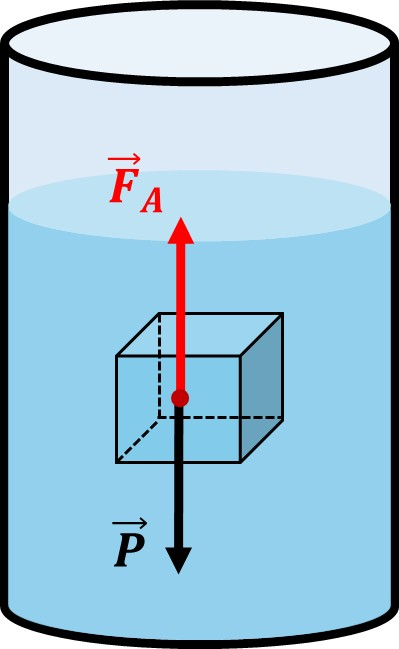
\includegraphics[scale=0.5]{figs/G10-BAI11-15}
		\end{center}
		Câu trả lời: $F_A=P=\rho gV$.
		\item GV đặt vấn đề, bây giờ nếu thay khối chất lỏng lập phương trên bằng một vật khác có cùng thể tích chiếm chỗ thì lực đẩy của chất lỏng xung quanh vẫn không đổi. Điều đó là hiển nhiên vì cùng là các phần tử chất lỏng bao quanh thể tích đó.
		\item Từ đó, GV rút ra biểu thức tổng quát của lực đẩy Archimedes do chất lỏng tác dụng lên vật chìm trong nó.
		\item GV chuyển giao Ví dụ 5 và Ví dụ 6 cho HS.
	\end{itemize}
	\textit{\underline{* HS thực hiện nhiệm vụ học tập}}\\
	HS chú ý lắng nghe và tích cực trả lời các câu hỏi gợi ý của GV.\\
	HS thực hiện Ví dụ 5 - 6.\\
	\textit{\bfseries\underline{* HS báo cáo kết quả nhiệm vụ học tập}}\\
	GV lần lượt mời HS trả lời câu hỏi và lên bảng giải bài tập Ví dụ 5 - 6.
}
\hoatdong{
	Luyện tập.
}
{
HS sử dụng phương pháp động lực học để giải quyết các bài toán đặc trưng.
}
{
	Bài tập cá nhân của học sinh.
}
{
	\textit{\underline{GV chuyển giao nhiệm vụ học tập}}\\
	GV lần lượt chuyển giao từng bài tập, yêu cầu HS hoạt động cá nhân để giải.\\
	\textit{\underline{HS thực hiện nhiệm vụ học tập}}\\
	HS \textit{(làm việc cá nhân)}:  Giải bài tập trong phiếu bài tập được GV giao. 
	
	GV: Theo dõi để phát hiện các HS gặp khó khăn, từ đó đưa ra sự định hướng, hỗ trợ phù hợp cho mỗi HS.\\
	\textit{\underline{HS báo cáo kết quả thực hiện nhiệm vụ học tập}}\\
	GV: Mời HS lên bảng giải bài tập.
	
	HS: Đặt câu hỏi, góp ý.
	
	GV: Chỉnh lí, hợp thức hoá kiến thức.
}
\section{HỒ SƠ DẠY HỌC}
\subsection{NỘI DUNG DẠY HỌC}
\begin{enumerate}[label=\bfseries\Roman*.]
	\item \textbf{LỰC HẤP DẪN}
	\begin{enumerate}[label=\bfseries\arabic*.]
		\item \textbf{Lực hấp dẫn:} mọi vật trong vũ trụ đều hút nhau với một lực gọi là lực hấp dẫn.
		\item \textbf{Định luật vạn vật hấp dẫn:} lực hấp dẫn giữa hai chất điểm tỉ lệ thuận với tích hai khối lượng của chúng và tỉ lệ nghịch với bình phương khoảng cách giữa chúng.
		$$F_{\mathrm{hd}}=G\dfrac{m_1m_2}{r^2}.$$
		Trong đó:
		\begin{itemize}
			\item $m_1$, $m_2$ là khối lượng của hai vật $\left(\si{\kilogram}\right)$;
			\item $r$ là khoảng cách giữa hai vật $\left(\si{\meter}\right)$;
			\item  $G=\SI{6.67E-11}{\newton\cdot\meter^2/\kilogram^2}$ là hằng số hấp dẫn.
		\end{itemize}
		\textit{\textbf{* Chú ý:} Phạm vi áp dụng của định luật
		\begin{itemize}
			\item Khoảng cách giữa các vật rất lớn so với kích thước giữa chúng.
			\item Các vật đồng chất và có dạng hình cầu, khi ấy $r$ là khoảng cách giữa 2 tâm và lực hấp dẫn nằm trên đường nối 2 tâm và ở 2 tâm đó.
		\end{itemize}}
	\item \textbf{Trọng lực là trường hợp riêng của lực hấp dẫn}\\
	Trọng lực của một vật là lực hấp dẫn giữa Trái Đất và vật đó. Độ lớn trọng lực:
	$$P=G\dfrac{mM}{\left(R+h\right)^2}.$$
	Trong đó:
	\begin{itemize}
		\item $m$ là khối lượng của vật $\left(\si{\kilogram}\right)$;
		\item $M$ là khối lượng Trái Đất $\left(\si{\kilogram}\right)$;
		\item $R$ là bán kính Trái Đất $\left(\si{\meter}\right)$;
		\item $h$ là độ cao của vật so với mặt đất $\left(\si{\meter}\right)$.
	\end{itemize}
	Gia tốc rơi tự do:
	$$g=\dfrac{GM}{\left(R+h\right)^2}$$
	$$\Rightarrow P=mg.$$
	Gia tốc rơi tự do phụ thuộc vào độ cao $h$ và vĩ độ địa lý.
	\end{enumerate}
	\item \textbf{LỰC MA SÁT}
	\begin{enumerate}[label=\bfseries\arabic*.]
		\item \textbf{Lực ma sát trượt:} xuất hiện khi một vật trượt trên mặt vật khác và có tác dụng cản trở chuyển động của vật.\\
		\textbf{* Đặc điểm của lực ma sát trượt:}
		\begin{itemize}
			\item Xuất hiện ở mặt tiếp xúc của vật đang trượt trên một bề mặt.
			\item Có hướng ngược với hướng của vận tốc (ngược hướng chuyển động).
			\item Có độ lớn tỉ lệ với độ lớn của áp lực.
			\item Lực ma sát trượt không phụ thuộc vào diện tích mặt tiếp xúc và vận tốc của vật mà chỉ phụ thuộc vào áp lực, vật liệu và tình trạng của hai mặt tiếp xúc.
			\item Độ lớn lực ma sát trượt:
			$$F_{\text{ms}}=\mu N.$$
			Trong đó:
			\begin{itemize}
				\item $N$ là áp lực của vật lên mặt tiếp xúc $\left(\si{\newton}\right)$;
				\item $\mu$ là hệ số ma sát trượt, phụ thuộc vào vật liệu và tình trạng hai mặt tiếp xúc.
			\end{itemize}
		\end{itemize}
		\item \textbf{Lực ma sát lăn:}\\
		Xuất hiện ở chỗ tiếp xúc khi vật lăn trên bề mặt.
		\item \textbf{Lực ma sát nghỉ}\\
		Xuất hiện ở mặt tiếp xúc của vật với bề mặt để giữ cho vật đứng yên trên bề mặt đó khi vật bị một lực tác dụng nhưng chưa chuyển động.\\
		\textbf{* Đặc điểm:}
		\begin{itemize}
			\item Có hướng ngược với hướng của lực tác dụng theo phương song song với mặt tiếp xúc.
			\item Có độ lớn bằng độ lớn của lực tác dụng theo phương song song với mặt tiếp xúc khi vật chưa chuyển động.
			\item Có độ lớn cực đại, lực ma sát nghỉ cực đại lớn hơn lực ma sát trượt.
		\end{itemize}
	\end{enumerate}
	\item \textbf{LỰC CĂNG DÂY}\\
	Khi một sợi dây bị kéo căng, sẽ có lực tác dụng lên hai vật gắn với hai đầu dây, lực căng dây có đặc điểm:
	\begin{itemize}
		\item Điểm đặt là điểm mà đầu dây tiếp xúc với vật.
		\item Phương của lực là phương của sợi dây.
		\item Chiều hướng từ hai đầu dây vào điểm giữa của dây.
	\end{itemize}
	Với những dây có khối lượng không đáng kể thì lực căng ở hai đầu dây luôn có cùng độ lớn.
	\item \textbf{LỰC ĐẨY ARCHIMEDES}\\
	\begin{enumerate}[label=\bfseries \arabic*.]
		\item \textbf{Lực đẩy Archimedes} tác dụng lên vật có điểm đặt tại vị trí trùng với trọng tâm của phần chất lỏng bị vật chiếm chỗ, có phương thẳng đứng, có chiều từ dưới lên trên, có độ lớn bằng trọng lượng phần chất lỏng bị chiếm chỗ.
		$$F=\rho gV.$$
		Trong đó:
		\begin{itemize}
			\item $\rho$ là khối lượng riêng của chất lỏng $\left(\si{\kilogram/\meter^3}\right)$;
			\item $g$ là gia tốc trọng trường $\left(\si{\meter/\second^2}\right)$;
			\item $V$ là thể tích phần chất lỏng bị vật chiếm chỗ $\left(\si{\meter^3}\right)$.
		\end{itemize}
		\item \textbf{Khối lượng riêng}\\
		Khối lượng riêng của một chất được xác định bằng khối lượng của một đơn vị thể tích chất đó
		$$\rho=\dfrac{m}{V}.$$
		Trong đó:
		\begin{itemize}
			\item $m$ là khối lượng $\left(\si{\kilogram}\right)$;
			\item $V$ là thể tích $\left(\si{\meter^3}\right)$.
		\end{itemize}
	\end{enumerate}
\end{enumerate}
\subsection{CÁC VÍ DỤ MINH HỌA}
\setcounter{ex}{0}
% ======================================================================
\begin{ex}
	\immini{Một quả khúc côn cầu chuyển động với tốc độ \SI{20.0}{\meter/\second} sau một cú đánh. Quả khúc côn cầu này vẫn có thể trượt chậm dần đều một đoạn \SI{1.20E2}{\meter} trên mặt sân trước khi dừng lại. Xác định hệ số ma sát trượt của nó với mặt sân.}{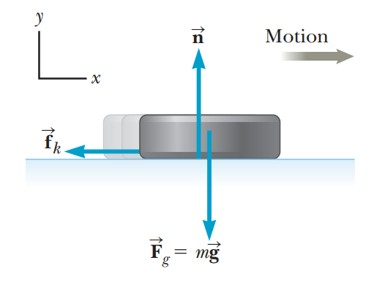
\includegraphics[scale=0.5]{figs/G10-BAI11-16}}
	\loigiai{}
\end{ex}
% ======================================================================
\begin{ex}
	Một tủ lạnh có khối lượng \SI{120}{\kilogram} được kéo trượt trên mặt sàn nằm ngang. Biết hệ số ma sát trượt giữa tủ lạnh và mặt sàn là $\mu=0,3$.
	\begin{enumerate}[label=\alph*)]
		\item Biết lực kéo có phương nằm ngang và có độ lớn \SI{500}{\newton}. Tính gia tốc của tủ lạnh.
		\item Sau thời gian \SI{10}{\second} kể từ lúc kéo, người ta buông tay. Tủ lạnh sẽ chuyển động với gia tốc bằng bao nhiêu? Tính tổng quãng đường tủ lạnh đi được.
	\end{enumerate}
	\loigiai{}
\end{ex}
% ======================================================================
\begin{ex}
	\immini{Để đẩy chiếc thùng nặng, cần tác dụng một lực kéo theo phương ngang có giá trị tối thiểu \SI{300}{\newton} để thắng lực ma sát nghỉ. Nếu người kéo thùng với lực \SI{35}{\newton} và người kia đẩy thùng với lực \SI{260}{\newton} thì có thể làm dịch chuyển thùng được không?
	}
	{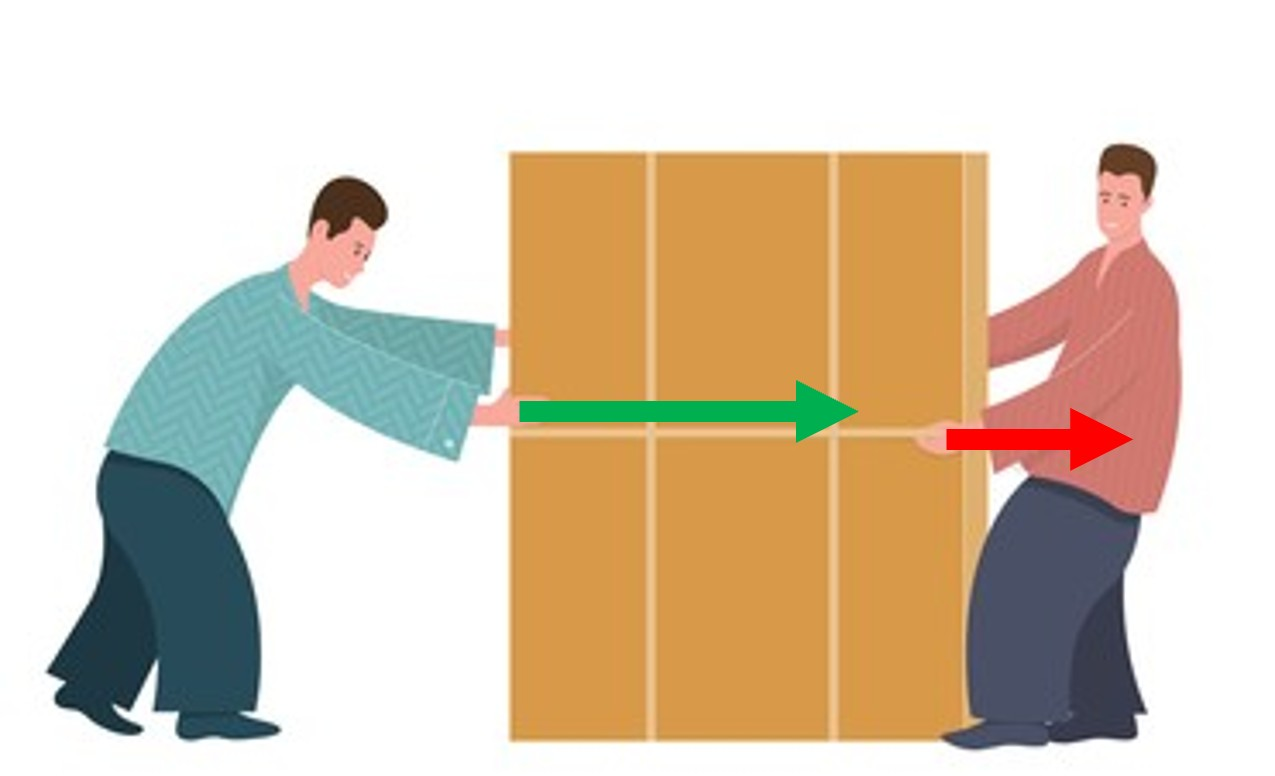
\includegraphics[scale=0.5]{figs/G10-BAI11-17}}
	\loigiai{}
\end{ex}
\begin{ex}
	\immini{Một tên trộm đang trèo tường để đào thoát bằng một sợi dây như hình minh họa. Trọng lượng của tên trộm này là $\SI{600}{\newton}$. 
		\begin{enumerate}[label=\alph*)]
			\item Xác định lực căng trên mỗi dây.
			\item Nếu điểm treo của sợi dây nằm ngang được đặt ở vị trí cao hơn trên tường thì lực căng của sợi dây bên kia sẽ thay đổi như thế nào?
		\end{enumerate}
	}
	{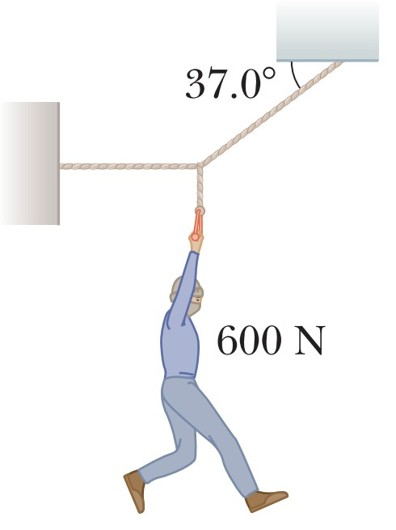
\includegraphics[scale=0.4]{figs/G10-BAI11-18}}
\end{ex}
\begin{ex}
	\immini{Vào năm 231, một chiếc vương miện mới đã được chế tạo cho Vua Hiero II. Nhà vua yêu cầu Archimedes xác định liệu vương miện có phải được sử dụng vàng ròng hay được pha thêm bạc bởi một người thợ bất lương. Archimedes phải giải quyết vấn đề mà không được làm hư hại chiếc vương miện, do đó ông tiến thành thí nghiệm như hình minh họa bên. }
	{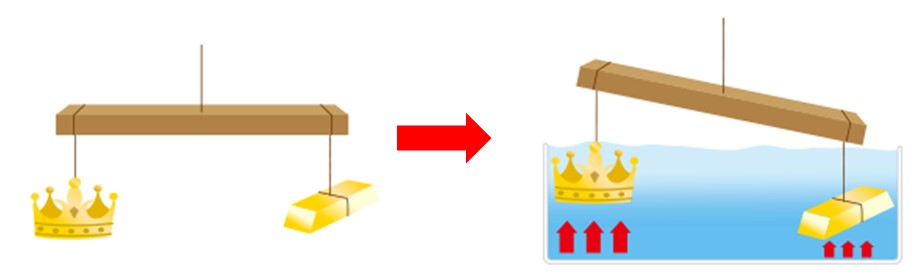
\includegraphics[scale=0.6]{figs/BTMASAT-8}}
	Dựa vào kiến thức đã học, em hãy giải thích cơ sở khoa học của thí nghiệm do Archimedes thực hiện. Biết rằng bạc có khối lượng riêng nhỏ hơn vàng.
\end{ex}
\begin{ex}
	\immini{Một khối gỗ hình hộp chữ nhật có diện tích đáy $S=\SI{40}{\centi\meter^2}$ và cao $h=\SI{10}{\centi\meter}$. Khối lượng của khối gỗ $m=\SI{160}{\gram}$. Khối lượng riêng của nước là $\rho=\SI{1000}{\kilogram/\meter^3}$. Thả khối gỗ vào nước, khối gỗ nổi lơ lửng trên mặt nước như hình vẽ. Tìm chiều cao của phần gỗ nổi trên mặt nước.}
	{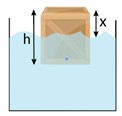
\includegraphics[scale=0.7]{figs/BTMASAT-7}	
	}
\end{ex}